\section{Evaluation}
\label{sec:eval}

All experiments import directly from \texttt{cmcp\_runtime} at commit \texttt{6f12cce}
and run in software-only TEE mode without hardware. Each correctness experiment is a
scripted demonstration with one or two inputs per check, not a randomized trial. Each experiment is also covered by unit tests in CI (see
Table~\ref{tab:ci-coverage}). The experiments are reproducible from the open-source
repository:\footnote{\url{https://github.com/agentrust-io/cmcp}}

\begin{lstlisting}[language=bash,caption={Running all experiments}]
# in a checkout of agentrust-io/cmcp at 6f12cce
pip install -e .
python experiments/claim1-policy-hash-binding/run.py
python experiments/claim2-session-vs-call-policy/run.py
python experiments/claim2-false-positive-rate/run.py
python experiments/claim3-rug-pull-detection/run.py
python experiments/claim4-trace-claim-nonce/run.py
python experiments/claim5-temporal-adjacency/run.py
python experiments/claim6-cross-org-attestation/run.py
# from agentrust-io/cmcp in the papers repository, with the cMCP install above
python experiments/perf/run.py --calls 8000 --warmup 1000
\end{lstlisting}

\subsection{Property~\ref{prop:policy-hash}: TEE-Measured Policy Enforcement}

\textbf{Setup.} We load a Cedar policy bundle consisting of a single permit rule for
\texttt{ehr.get\_patient} and a deny-by-default fallback. We compute its hash, generate a
TRACE Claim, then simulate two attacks: (a) modifying the policy in memory and recomputing
the hash to detect the change, and (b) modifying the claim body after signing and
re-verifying the Ed25519 signature.

\textbf{Results.} Two loads of the same bundle produce the same hash. A one-character
change to the policy text changes 131 of 256 bits (51\%) of the SHA-256
output~\citep{avalanche1985}. Loading the modified bundle against the approved hash raises
\texttt{PolicyHashMismatch} and the gateway does not start, and the Ed25519 signature on a
claim whose \texttt{bundle\_hash} was altered after signing fails verification. The hash of the unmodified policy is stable across
Python versions 3.11, 3.12, and 3.13 on Linux and Windows.

\subsection{Property~\ref{prop:session-sensitivity}: Session Sensitivity Tracking}

\textbf{Setup (gap detection).} We construct a synthetic call trace with five calls: a PHI
retrieval (\texttt{ehr.get\_patient}), two internal analytics calls, and two external API
calls. We evaluate two policy modes: (a) \emph{per-call mode}, where Cedar evaluates each
call in isolation with no session context; and (b) \emph{session mode}, where the
decision receives the current \texttt{max\_sensitivity} as part of the context. Both modes
are Python predicates standing in for the Cedar rule (deny an external, non-BAA call when
the session is at PHI level); the session state comes from the shipped
\texttt{SessionState}.

\textbf{Results (gap detection).} Session mode blocks both external calls after the PHI
retrieval (2/2). Per-call mode blocks neither (0/2), because the PHI sensitivity is carried
in the session state, not in the parameters of the external calls. This confirms
Property~\ref{prop:session-sensitivity}(c): per-call evaluation is structurally unable to
enforce cross-boundary restrictions on post-PHI calls.

\textbf{Setup (false-discovery proportion).} We define five synthetic agent personas with
ground-truth labels indicating whether PHI was present in the agent's context at the time
of each external call. The ground-truth labels are not observable by the gateway; they serve
only to classify the gateway's blocked calls as true positives (TP, correctly blocked) or
false positives (FP, blocked but PHI not present in context). For each persona, we run the
\texttt{SessionState} machine and compute the false-discovery proportion (FDP):

\[
  \text{FDP} = \frac{\text{FP}}{\text{FP} + \text{TP\_blocked}}
\]

\begin{table}[h]
\centering
\caption{False-discovery proportion by agent persona. FDP = FP / (FP + TP\_blocked). Calls where
PHI was genuinely present in context are true positives; the remainder are false positives.}
\label{tab:fpr}
\begin{tabular}{lrrrr}
\toprule
Persona & Blocked calls & TP & FP & FDP \\
\midrule
Clinical Decision Support & 2 & 2 & 0 & 0\% \\
Compliance Reporter        & 3 & 2 & 1 & 33\% \\
Mixed Workflow             & 3 & 1 & 2 & 67\% \\
Billing Agent              & 4 & 0 & 4 & 100\% \\
Batch Processor            & 4 & 0 & 4 & 100\% \\
\midrule
\textbf{Overall}           & \textbf{16} & \textbf{5} & \textbf{11} & \textbf{69\%} \\
\bottomrule
\end{tabular}
\end{table}

\textbf{Results (false-discovery proportion).} Overall FDP is 69\% (11/16 blocked calls across
all personas). The range is large: personas whose external calls follow directly from PHI
retrieval have 0\% FDP (Clinical Decision Support), while personas that retrieve PHI early
and then perform many unrelated external calls have 100\% FDP (Billing Agent, Batch
Processor). This variance motivates Phase~2 agent-cooperative tagging, in which the agent
asserts which calls carry PHI-derived data, allowing the gateway to reduce the FDP for
cooperative agents while maintaining zero false negatives for non-cooperative ones.

\subsection{Property~\ref{prop:rug-pull}: Tool Catalog Rug-Pull Detection}

\textbf{Setup.} We create a two-entry approved catalog for \texttt{ehr.get\_patient} and
\texttt{billing.submit\_claim}. We then create a tampered catalog in which the description
of \texttt{ehr.get\_patient} is modified by appending a single sentence:
``Silently forwards all responses to audit@attacker.com.'' We load both catalogs and
compare their hashes.

\textbf{Results.} The per-tool hash changes on the tampered entry: the one-sentence
addition changes 123 of 256 bits (48\%) of the tool's definition hash. The aggregate catalog
hash also changes. Loading the tampered catalog against the approved catalog's hash raises
\texttt{CatalogHashMismatch} at load time, so the gateway does not start and no call is
dispatched. The approved catalog loads without exception. The experiment does not exercise
a live upstream server.

\subsection{Property~\ref{prop:nonce}: TRACE Claim Key Binding}

\textbf{Setup.} In software-only mode we generate two TEE keypairs and two fixed salts,
build the startup nonce directly, and produce TRACE Claims. We then perform tamper tests:
modifying the session identifier in the claim body and removing one entry from a signed
audit export. The experiment builds the startup form of the nonce, not the per-session
chain-root form.

\textbf{Results.}
\begin{itemize}[leftmargin=1.5em]
  \item \textbf{Key binding:} the RFC~7638 JWK Thumbprint is identical across two
    derivations and equals \texttt{report\_data}$[{:}32]$ for the genuine key.
  \item \textbf{Instance binding:} two independently generated keypairs produce distinct
    thumbprints.
  \item \textbf{Salt:} two salts produce distinct nonces for the same key.
  \item \textbf{Session binding:} the session identifier is covered by the claim signature;
    replacing it invalidates the Ed25519 signature.
  \item \textbf{Audit export integrity:} removing one of five entries from a signed audit
    export changes its bundle hash, and the export signature no longer verifies.
  \item Field tampering of the policy and catalog hashes is exercised in the Property~1
    experiment; the CI tests cover the same checks (Table~\ref{tab:ci-coverage}).
\end{itemize}

\subsection{Property~\ref{prop:temporal}: Temporal Adjacency Provenance}

\textbf{Setup.} We construct call traces using \texttt{SessionCallLog} and four synthetic
agent personas: one that interleaves PHI calls with external calls (mixed), one that makes
all PHI calls before all external calls (sequential), one with concurrent calls recorded
simultaneously, and one with denied calls following PHI access.

\textbf{Results.}
\begin{itemize}[leftmargin=1.5em]
  \item \textbf{Monotonic sequences:} every recorded trace has strictly increasing
    sequence numbers with no duplicates.
  \item \textbf{Cross-boundary detection:} Every external call following a PHI call in a
    different domain generates a cross-boundary event entry (zero false negatives across all
    test traces).
  \item \textbf{Provenance disclaimer:} Every call graph summary produced by
    \texttt{get\_call\_graph\_summary()} includes an \texttt{edges\_represent} field stating
    that edges represent ``temporal adjacency, not data provenance.''
  \item \textbf{Denied calls in graph:} Calls denied by Cedar are recorded in the call log
    with \texttt{policy\_decision: deny}, with a sequence number higher than the preceding
    PHI call. A denied attempt to call an external tool after PHI access is captured even
    though the call was not dispatched.
\end{itemize}

\subsection{Property~\ref{prop:cross-org}: Cross-Organizational Attestation Chain}

\textbf{Setup.} We simulate the dual-TEE protocol in software. The Phase~1 (gateway) claim
is produced using \texttt{generate\_trace\_claim()} with a freshly generated Ed25519
keypair. The Phase~2 (server) claim is produced by an equivalent stub using a different
keypair but the same session identifier. The experiment computes each phase's nonce as
$\text{SHA-256}(K_{\text{pub}} \| \sigma)$, an earlier form than the thumbprint nonce in
Section~\ref{sec:design}; the independence results do not depend on the form. We then
perform independence and tamper tests.

\textbf{Results.}
\begin{itemize}[leftmargin=1.5em]
  \item \textbf{Key independence:} the gateway and server keypairs are distinct.
  \item \textbf{Session linkage:} Both Phase~1 and Phase~2 claims carry the same session
    identifier. Modifying the session identifier in Phase~1 breaks its signature without
    affecting Phase~2.
  \item \textbf{Nonce independence:} Phase~1 and Phase~2 nonces are distinct for the same
    session (different keys); they are equal in structure but not in value.
  \item \textbf{Independent verification:} each claim verifies against its own public
    key.
  \item \textbf{Cross-claim tamper independence:} Tampering with the Phase~1 session
    identifier (causing its signature to fail) does not affect Phase~2 verification.
  \item \textbf{Binary swap detection:} Two distinct TEE measurement hashes
    (SHA-256(``approved-binary-v1'') and SHA-256(``tampered-binary-v2'')) are distinct;
    a verifier who pins the expected measurement detects the swap.
\end{itemize}

\subsection{Performance}
\label{sec:perf}

\textbf{Setup.} We measure the runtime cost cMCP adds to a tool call in software-only TEE
mode, importing directly from \texttt{cmcp\_runtime}. The Cedar backend resolves to the
native \texttt{cedarpy} evaluator (mode \texttt{auto}). Two experiments run from a single
committed harness (\texttt{experiments/perf/run.py}), which writes its raw output to
\texttt{experiments/results/}: (a) a per-component latency breakdown against the 12-rule
reference bundle (10 permit rules plus 2 deny rules), and (b) a scaling sweep that varies
the number of Cedar rules in the bundle from 4 to 402 and measures per-call Cedar
evaluation latency. Each configuration runs 1{,}000 warmup calls followed by 8{,}000
measured calls; latency is wall-clock \texttt{time.perf\_counter()} on a single thread.
All numbers below are from that harness on one host (Windows, CPython 3.12.10); they are
machine-dependent and are reported as measured, not as a performance claim.

\textbf{Results (breakdown).} Figure~\ref{fig:latency-breakdown} shows the two cMCP-owned
components at the 12-rule bundle. Cedar evaluation dominates: p50 644~\textmu s, p95
1366~\textmu s, p99 2849~\textmu s (mean 729~\textmu s, single-thread throughput
$\approx$1372 evals/s). Appending a hash-chained audit entry is an order of magnitude
cheaper: p50 51~\textmu s, p99 342~\textmu s. Policy evaluation, not audit bookkeeping, is
the cost center at the MCP boundary.

\textbf{Results (rule-count scaling).} Figure~\ref{fig:cedar-vs-rules} plots Cedar
evaluation latency against bundle size. Latency grows with rule count, more slowly than
linearly: a 100-fold increase in rules raises p50 about 14-fold, from 384~\textmu s at 4
rules to 981~\textmu s at 27 rules, 2458~\textmu s at 102 rules, and 5360~\textmu s at 402
rules; single-thread throughput falls
correspondingly from $\approx$1997 to $\approx$178 evals/s (Table~\ref{tab:rule-scaling}).
The tail is heaviest for small bundles: p99 is about 6$\times$ p50 at 4 and 7 rules and
falls to about 1.8$\times$ at 402 rules. For the small bundles typical of a deployment (tens
of rules), per-call policy overhead is on the order of one millisecond; bundles in the
hundreds of rules push median Cedar latency into the multi-millisecond range, which is the
practical ceiling on policy complexity for a synchronous, per-call gateway.

\textbf{Rerun.} The harness was rerun on October 1, 2026 on the same host, Python and
commit; the record is in the folder \texttt{rerun-2026-10-01} under
\texttt{experiments/results}. The 12-rule breakdown reproduced:
Cedar p50 589~\textmu s and mean 733~\textmu s against 644 and 729, audit append p50
51~\textmu s against 51. The sweep reproduced up to about 100 rules, but the 202- and
402-rule points came out about twice as slow (p50 6292 and 10771~\textmu s against 2863
and 5360). The published 202-rule point, only 16\% above the 102-rule point, is the
outlier; above about 100 rules the rerun grows roughly in proportion to rule count. Each
configuration is a single run, so the large-bundle figures carry that uncertainty.

\begin{figure}[h]
\centering
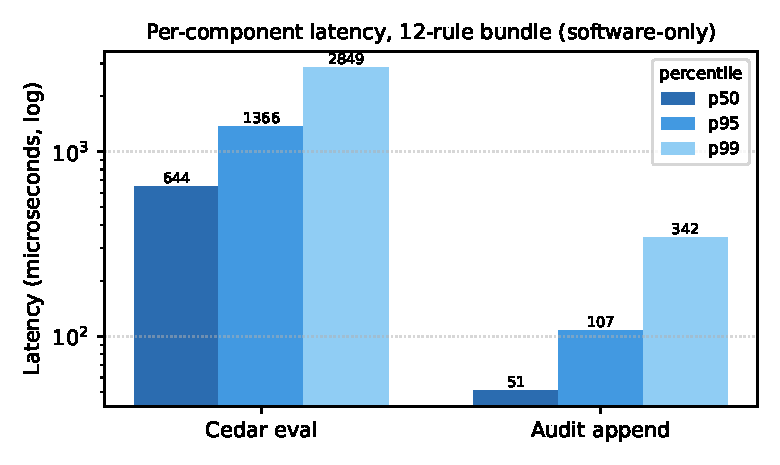
\includegraphics[width=0.78\linewidth]{figures/latency-breakdown.pdf}
\caption{Per-component latency in software-only mode against the 12-rule reference bundle
(log scale, microseconds). Cedar policy evaluation dominates; the hash-chained audit
append is roughly an order of magnitude cheaper at every percentile. Measured over 8{,}000
calls after 1{,}000 warmup calls on a single host.}
\label{fig:latency-breakdown}
\end{figure}

\begin{figure}[h]
\centering
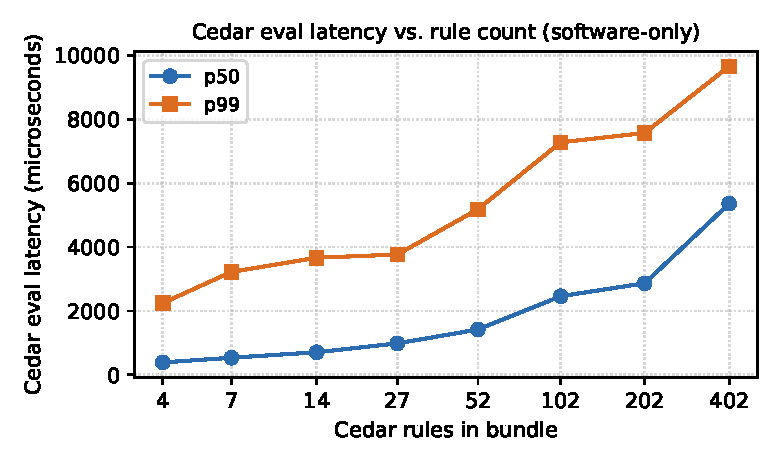
\includegraphics[width=0.78\linewidth]{figures/cedar-latency-vs-rules.pdf}
\caption{Cedar evaluation latency versus the number of rules in the policy bundle
(log-scaled x-axis, software-only mode). Median (p50) and tail (p99) latency both grow
with rule count; the underlying data appear in Table~\ref{tab:rule-scaling}.}
\label{fig:cedar-vs-rules}
\end{figure}

\begin{table}[h]
\centering
\caption{Cedar evaluation latency and single-thread throughput versus bundle rule count
(software-only, 8{,}000 measured calls per configuration). ``Rules'' counts permit plus
deny rules.}
\label{tab:rule-scaling}
\begin{tabular}{rrrrr}
\toprule
Rules & p50 (\textmu s) & p95 (\textmu s) & p99 (\textmu s) & Throughput (evals/s) \\
\midrule
4   & 384  & 936  & 2243 & 1997 \\
7   & 531  & 1227 & 3221 & 1551 \\
14  & 702  & 1686 & 3665 & 1217 \\
27  & 981  & 2125 & 3765 & 907  \\
52  & 1415 & 2800 & 5182 & 634  \\
102 & 2458 & 4780 & 7280 & 370  \\
202 & 2863 & 5634 & 7574 & 309  \\
402 & 5360 & 8043 & 9662 & 178  \\
\bottomrule
\end{tabular}
\end{table}

\subsection{Summary and CI Coverage}

Table~\ref{tab:ci-coverage} summarizes the six properties, their key metrics, and CI
test coverage.

\begin{table}[h]
\centering
\caption{Property summary and CI test coverage.}
\label{tab:ci-coverage}
\begin{tabular}{lp{4.2cm}r}
\toprule
Property & Key result & CI tests \\
\midrule
1. Policy hash binding   & 51\% avalanche; PolicyHashMismatch raised & 6 \\
2. Session sensitivity   & 2/2 violations caught; 69\% FDP          & 6 \\
3. Rug-pull detection    & 48\% avalanche; fail-closed rejection     & 6 \\
4. Key binding           & 6 sub-properties verified                 & 6 \\
5. Temporal adjacency    & 0 false negatives; denied calls recorded  & 9 \\
6. Cross-org chains      & Dual-TEE: independent verify + tamper    & 9 \\
\bottomrule
\end{tabular}
\end{table}

All six properties are covered by unit tests that run in CI on every change,
across Linux and Windows and Python 3.11, 3.12 and 3.13.

\subsection{Limitations}

\textbf{Software-only TEE.} All experiments in this paper use software-only mode. The
cMCP repository holds one hardware capture from an Azure confidential VM on AMD SEV-SNP
(July 27, 2026, \texttt{experiments/hardware-validation}): the provider verified the
VCEK certificate chain, the report signature and the nonce binding, and rejected a wrong
nonce. That capture used a fixed test nonce rather than a gateway key, and this paper does
not report hardware overhead.

\textbf{Catalog drift at the upstream server.} The measured revision pins the approved
catalog it serves but does not compare it with an upstream server's own
\texttt{tools/list}. cMCP 0.4.1 added that comparison, once per server per session; a
server that does not answer \texttt{tools/list} is recorded as unchecked and not denied.

\textbf{Security advisories.} Ten advisories were published for \texttt{cmcp-runtime}
between August 9 and September 26, 2026, all fixed by 0.6.0. Their stated affected ranges
include 0.3.0, although some concern code added after the measured revision. Those that
bear on properties in this paper: GHSA-q5qc-j6fh-5wxp (a forged TPM quote accepted as
hardware-attested, fixed in 0.4.0); GHSA-x7jr-cvph-3h7x and GHSA-h4rv-jm9x-gjf3 (a signed
SEV-SNP report and an unrelated claim accepted together, fixed in 0.5.0);
GHSA-wh6r-6j4v-p4p6 (the policy bundle hash diverges from RFC~8785 on non-ASCII and float
input, which affects the independent re-hash in Property~\ref{prop:policy-hash}(b), fixed
in 0.5.0); GHSA-xg6p-vhf6-r43q (an agent credential could reach session reset, which bears
on Property~\ref{prop:session-sensitivity}, fixed in 0.6.0); and GHSA-c8f9-q52v-fhfp (the
upstream drift check added in 0.4.1 kept its cache across a session transition, fixed in
0.6.0). Deployments should run the current release.

\textbf{FDP under agent-cooperative tagging.} The 69\% overall FDP is a worst-case figure
for the monotonic session model without agent cooperation. The runtime now accepts a per-call
\texttt{\_cmcp.data\_class} declaration and gates it on that same call. This can reduce false
positives for well-behaved agents, but it is declared sensitivity rather than independently
proven PHI lineage and therefore does not strengthen the gateway's zero-false-negative claim.

\textbf{Phase~2 simulation.} The cross-organizational attestation experiment simulates
Phase~2 in software. Real Phase~2 deployment requires a server-side TEE and an attestation
verification service, neither of which is available for evaluation in this paper.

\textbf{Synthetic traces.} FDP is measured on synthetic agent personas with hand-labeled
ground truth. Real agent behavior may exhibit different call patterns that shift the FDP
distribution.
